%%%%%%%%%%%%%%%%%%%%%%%%%
%% Header for standard beamer presentation
%%
%%  PresentationHeader.tex
%%
%%%%%%%%%%%%%%%%%%%%%%%%%

\documentclass[english,10pt]{beamer}

%%%%%%%%%%%%%%%%%%%%
%% Include general header where common packages are defined
%%%%%%%%%%%%%%%%%%%%



%%%%%%%%%%%%%%%%%%%%%%%%%%
%% TEMPLATES
%%%%%%%%%%%%%%%%%%%%%%%%%%


% Simple Tabular

%\begin{tabular}{ |c|c|c| } 
% \hline
% cell1 & cell2 & cell3 \\ 
% cell4 & cell5 & cell6 \\ 
% cell7 & cell8 & cell9 \\ 
% \hline
%\end{tabular}





%%%%%%%%%%%%%%%%%%%%%%%%%%
%% Packages
%%%%%%%%%%%%%%%%%%%%%%%%%%


% general packages without options
\usepackage{amsmath,amssymb,amsthm,bbm}

% graphics
\usepackage{graphicx,transparent,eso-pic}

% text formatting
\usepackage[document]{ragged2e}
\usepackage{pagecolor,color,ulem,soul}








%%%%%%%%%%%%%%%%%%%%%%%%%%
%% Maths environment
%%%%%%%%%%%%%%%%%%%%%%%%%%

%\newtheorem{theorem}{Theorem}[section]
%\newtheorem{lemma}[theorem]{Lemma}
%\newtheorem{proposition}[theorem]{Proposition}
%\newtheorem{corollary}[theorem]{Corollary}

%\newenvironment{proof}[1][Proof]{\begin{trivlist}
%\item[\hskip \labelsep {\bfseries #1}]}{\end{trivlist}}
%\newenvironment{definition}[1][Definition]{\begin{trivlist}
%\item[\hskip \labelsep {\bfseries #1}]}{\end{trivlist}}
%\newenvironment{example}[1][Example]{\begin{trivlist}
%\item[\hskip \labelsep {\bfseries #1}]}{\end{trivlist}}
%\newenvironment{remark}[1][Remark]{\begin{trivlist}
%\item[\hskip \labelsep {\bfseries #1}]}{\end{trivlist}}

%\newcommand{\qed}{\nobreak \ifvmode \relax \else
%      \ifdim\lastskip<1.5em \hskip-\lastskip
%      \hskip1.5em plus0em minus0.5em \fi \nobreak
%      \vrule height0.75em width0.5em depth0.25em\fi}



%%%%%%%%%%%%%%%%%%%%
%% Idem general commands
%%%%%%%%%%%%%%%%%%%%

%\input{/Users/Juste/Documents/ComplexSystems/CityNetwork/Docs/Headers/GeneralCommands.tex}


\usetheme{Boadilla}

%\setbeamertemplate{footline}[text line]{}
%\setbeamercolor{structure}{fg=purple!50!blue, bg=purple!50!blue}

% cybergeo palette (from Clem server)
% #1C6F91, "#df691a", "#77c5ba", "orange", "#2db92d", "#e1ff2f", "#ff2313", "#bbab61
% redefine palette
\definecolor{cybblue}{HTML}{1C6F91}
\definecolor{cyborange}{HTML}{DF691A}
\definecolor{cybbluegreen}{HTML}{77C5BA}
\definecolor{cybgreen}{HTML}{2DB92D}
\definecolor{cybgreenyellow}{HTML}{E1FF2F}
\definecolor{cybred}{HTML}{FF2313}
\definecolor{cybglaucous}{HTML}{BBAB61}


\setbeamercolor{structure}{fg=cybblue}
\setbeamercolor{footline}{fg=orange, bg=orange}

\setbeamercovered{transparent}


\addtobeamertemplate{title page}{\hspace{-0.4cm}\vspace{-1.5cm}\includegraphics[height=1.2cm,width=1.2\textwidth]{template/bandeau3}\\
}{%
%\begin{textblock*}{150mm}(-1cm,-1.5cm)
%\end{textblock*}
}




\addtobeamertemplate{frametitle}{\hspace{-0.4cm}\vspace{-0.1cm}\includegraphics[height=1.2cm,width=1.2\textwidth]{template/bandeau3}\\
}{%
%\begin{textblock*}{150mm}(-1cm,-1.5cm)
%\end{textblock*}
}



% shortened command for a justified frame
\newcommand{\jframe}[2]{\frame{\frametitle{#1}\justify{#2}}}


\newcommand{\noun}[1]{\textsc{#1}}
\newcommand{\jitem}[1]{\item \begin{justify} #1 \end{justify} \vfill{}}
\newcommand{\sframe}[2]{\frame{\frametitle{#1} #2}}

\DeclareMathOperator{\Cov}{Cov}
\DeclareMathOperator{\Var}{Var}
\DeclareMathOperator{\E}{\mathbb{E}}
\DeclareMathOperator{\Proba}{\mathbb{P}}

\newcommand{\Covb}[2]{\ensuremath{\Cov\!\left[#1,#2\right]}}
\newcommand{\Eb}[1]{\ensuremath{\E\!\left[#1\right]}}
\newcommand{\Pb}[1]{\ensuremath{\Proba\!\left[#1\right]}}
\newcommand{\Varb}[1]{\ensuremath{\Var\!\left[#1\right]}}

% norm
\newcommand{\norm}[1]{\| #1 \|}

\newcommand{\indep}{\rotatebox[origin=c]{90}{$\models$}}


\usepackage{textpos}



%%%%%%%%%%%%%%%%%%%%%
%% Begin doc
%%%%%%%%%%%%%%%%%%%%%

\begin{document}



\title{Bibliom{\'e}trie Indirecte par Analyse de R{\'e}seaux Complexes}


\author{J.~Raimbault$^{1,2}$}

\institute{$^{1}$G{\'e}ographie-cit{\'e}s (UMR 8504 CNRS)\\
$^{2}$LVMT (UMR-T 9403 IFSTTAR)}

\date{S{\'e}minaire \textit{Cartha-G{\'e}o-Prisme}\\
Mercedi 17 f{\'e}vrier 2016}


\usebackgroundtemplate{%
  \AddToShipoutPicture*{
    \put(0,0){
        \parbox[b][\paperheight]{\paperwidth}{%
            \vfill
            \centering
            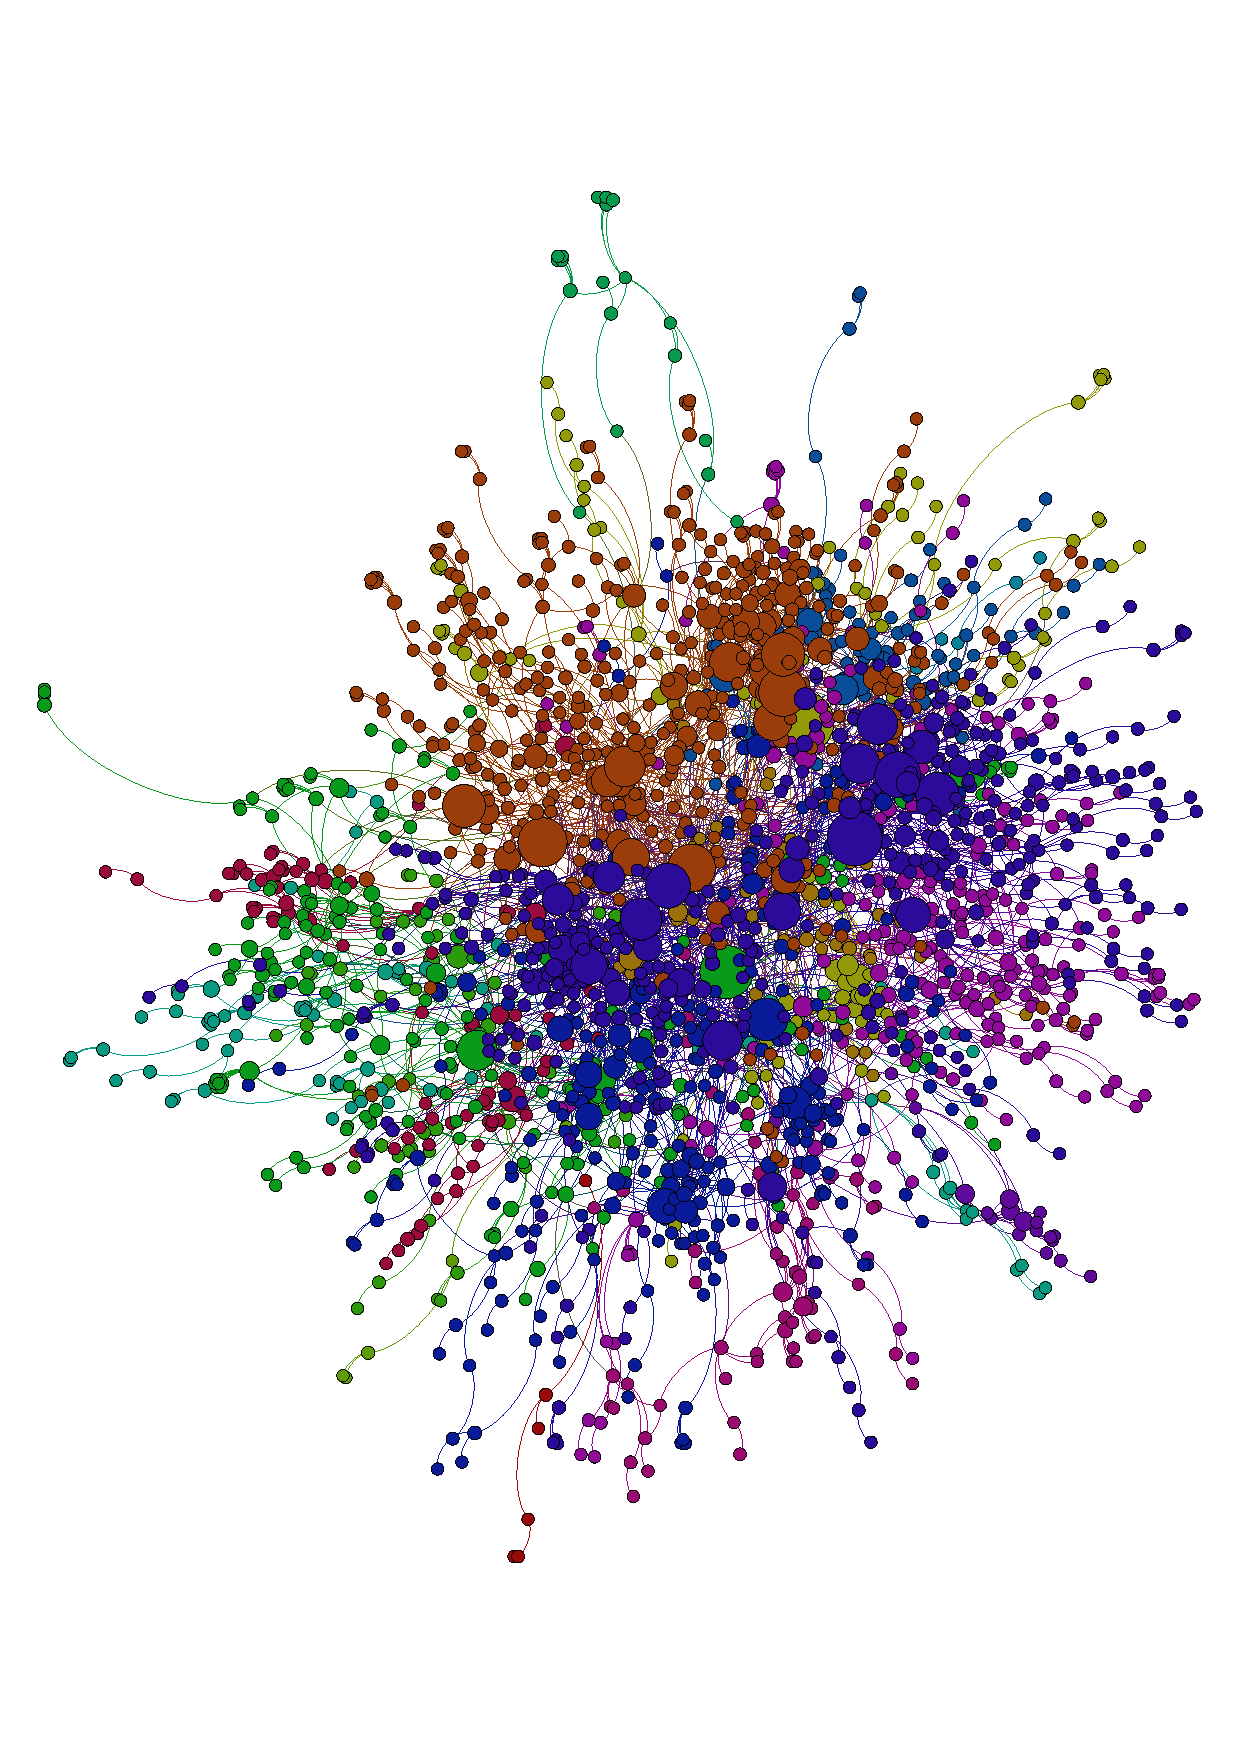
\includegraphics[width=\paperwidth]{figures/nw}%
            \vfill
        }
    }
    \put(0,0){%
        \transparent{0.9}\textcolor{white}{\rule{\paperwidth}{\paperheight}}
    }
}
  %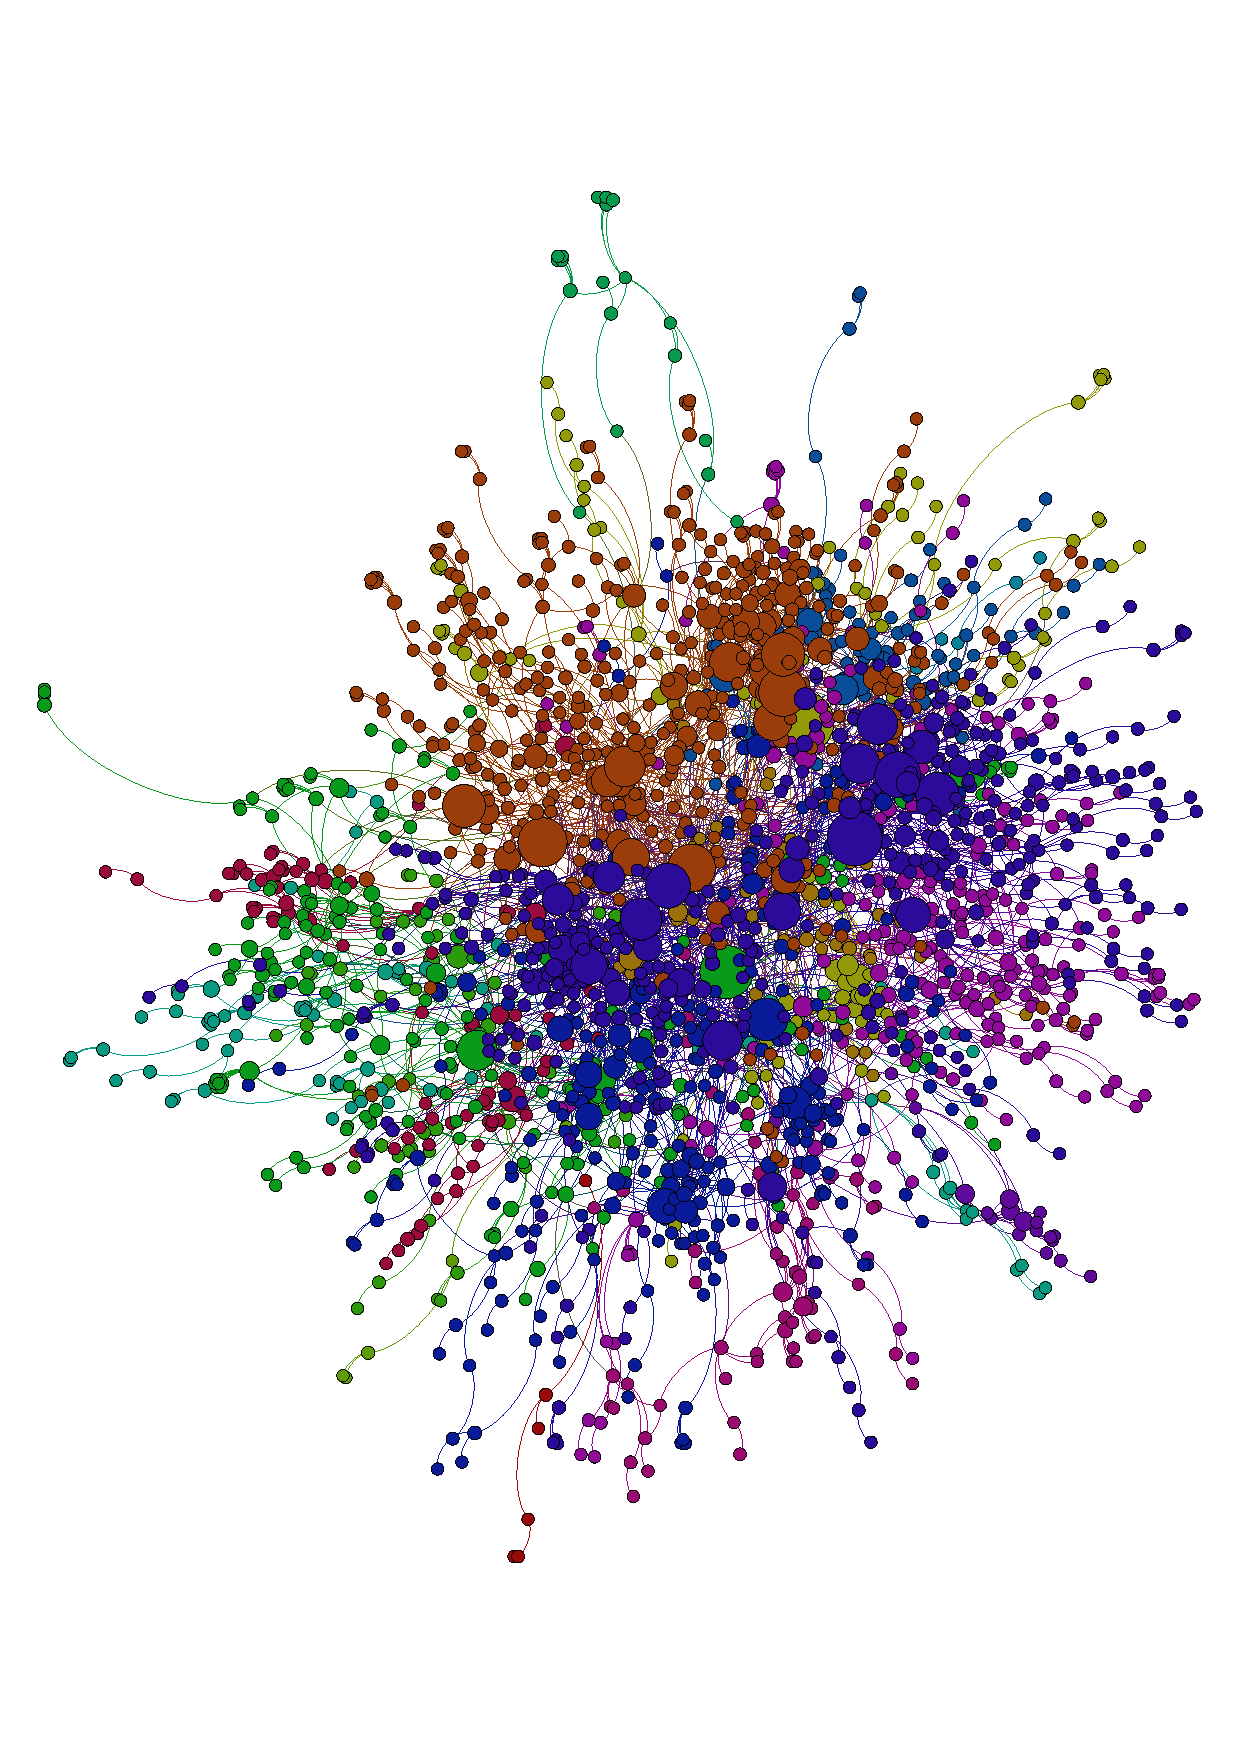
\includegraphics[width=1.5\paperwidth,height=1.5\paperheight]{figures/nw}
} 

%%%%%%%%%%%%%%%%%%%%%%%%%%%%%%%%
\begin{frame}
\titlepage
\end{frame}

% NO TOC
%\begin{frame}
%\tableofcontents
%\end{frame}
%%%%%%%%%%%%%%%%%%%%%%%%%%%%%%%%


\usebackgroundtemplate{}


\section{Introduction}

\jframe{Donn{\'e}es massives ?}{
\textit{Caract{\'e}ristiques n{\'e}c{\'e}ssaires possibles}
\bigskip
\begin{itemize}
\item \textbf{Taille relative} : algorithmes et/ou structures de stockage non-conventionnels
\bigskip
\item \textbf{Temps r{\'e}el} : traitement d'un flux de donn{\'e}es en temps r{\'e}el
\bigskip
\item \textbf{H{\'e}t{\'e}rog{\'e}n{\'e}it{\'e}} : diff{\'e}rentes sources, types, nature
\end{itemize}
}

\jframe{Cas d'{\'e}tude}{
Revue scientifique \textit{Cybergeo} : analyse bibliom{\'e}trique par approches vari{\'e}es

\bigskip

$\rightarrow$ Enjeu par rapport au positionnement de la revue : interdisciplinarit{\'e} ; contre une bibliom{\'e}trie quantitative pure en SHS

\bigskip

$\rightarrow$ Elaboration d'une approche par \textit{Hyperr{\'e}seau} : croisement du r{\'e}seau de citations au r{\'e}seau s{\'e}mantique.

\bigskip

$\rightarrow$ Donn{\'e}es difficiles d'acc{\`e}s : base {\`a} construire
 

}



\section{Collecte des donn{\'e}es}


\jframe{Collecte des donn{\'e}es}{
\textit{Crawling de donn{\'e}es semi-ouvertes : exemples en g{\'e}ographie}

\bigskip

Donn{\'e}es de mobilit{\'e} : statuts des stations Vlib en temps r{\'e}el (API)\cite{raimbault2015user}

\bigskip

\centering
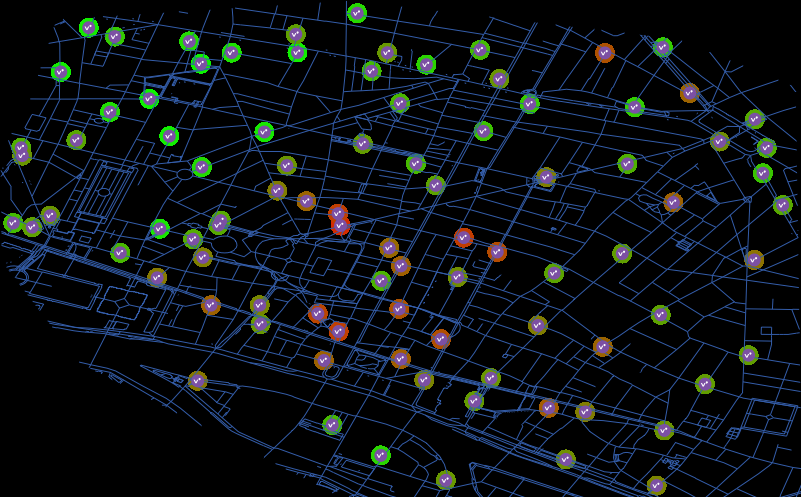
\includegraphics[width=0.7\textwidth]{figures/velib}



}

\jframe{Collecte des donn{\'e}es}{
\textit{Exemples en g{\'e}ographie (suite)}

\bigskip

Traffic routier : collecte de \textit{sytadin} (pas d'API : \textit{scrapping} n{\'e}c{\'e}ssaire)


\bigskip

\centering
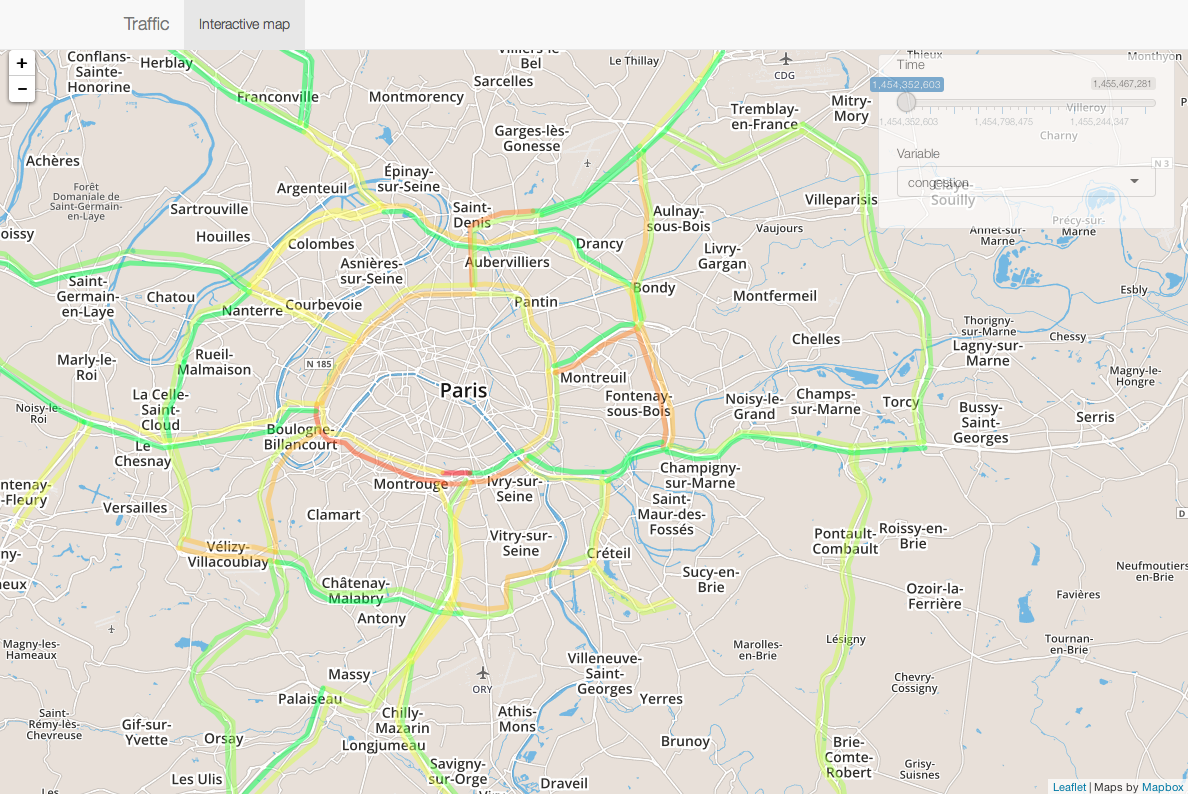
\includegraphics[width=0.8\textwidth]{figures/screen_appli}


\bigskip



}



\jframe{Collection des donn{\'e}es}{

\textbf{Donn{\'e}es des articles} : structuration, nettoyage et consolidation (sources diff{\'e}rentes)

\bigskip


\textbf{Donn{\'e}es de citation} : revue non r{\'e}f{\'e}renc{\'e}e par base ``classiques'' (de plus non libres !)

$\rightarrow$ \textit{crawling} de \texttt{google scholar} par utilisation de l'option ``\textit{cit{\'e} par}'' \cite{noruzi2005google}


\bigskip


\textbf{Donn{\'e}es textuelles} : besoin des r{\'e}sum{\'e}s pour l'ensemble des r{\'e}f{\'e}rences li{\'e}es

$\rightarrow$ utilisation de l'API Mendeley~\cite{mendeley} (gratuite mais non ouverte).


}



\jframe{Architecture de collecte des donn{\'e}es}{
\includegraphics[width=\textwidth]{figures/archi}
}





\section{M{\'e}thodes et R{\'e}sultats}

\subsection{R{\'e}seau des citations}


\jframe{Caract{\'e}ristiques du r{\'e}seau}{


$\rightarrow$ Apr{\`e}s raffinement, $\simeq$ 947 r{\'e}f{\'e}rences de cybergeo exploitables, sur $\simeq 1200$ ; certaines inexistantes, d'autres mal enregistr{\'e}es sur scholar% $\rightarrow$ possibilit{\'e} de compl{\'e}ter {\`a} la main (long...).

\smallskip

$\rightarrow$ \textit{418670 Noeuds et 570352 Liens ; Diam{\'e}tre : 9 ; Densit{\'e} : 3.25E-6 ; degr{\'e} moyen : 2.724284}

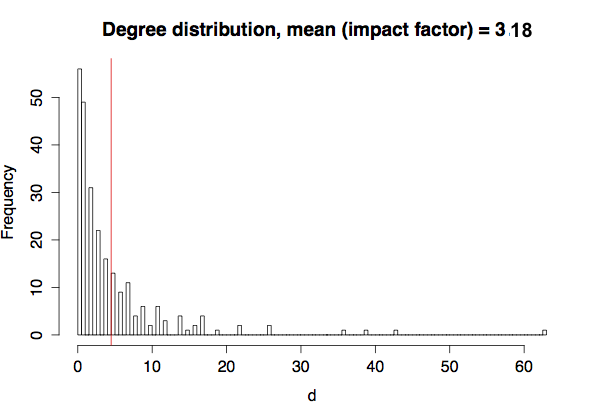
\includegraphics[width=0.8\textwidth]{figures/degreeDistrib.png}
}


\jframe{Degr{\'e}s : Loi rang-taille}{
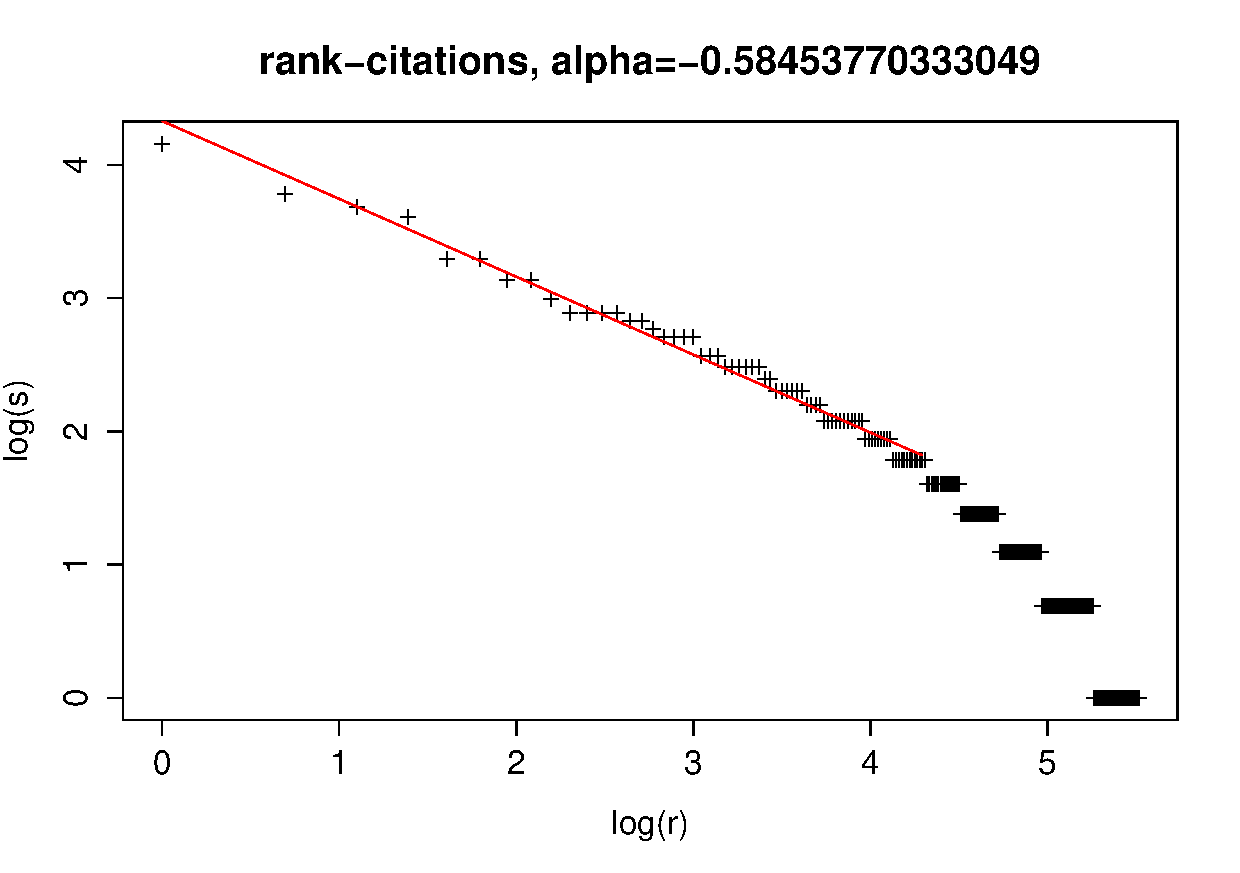
\includegraphics[width=0.52\textwidth]{figures/rankSize_fit}
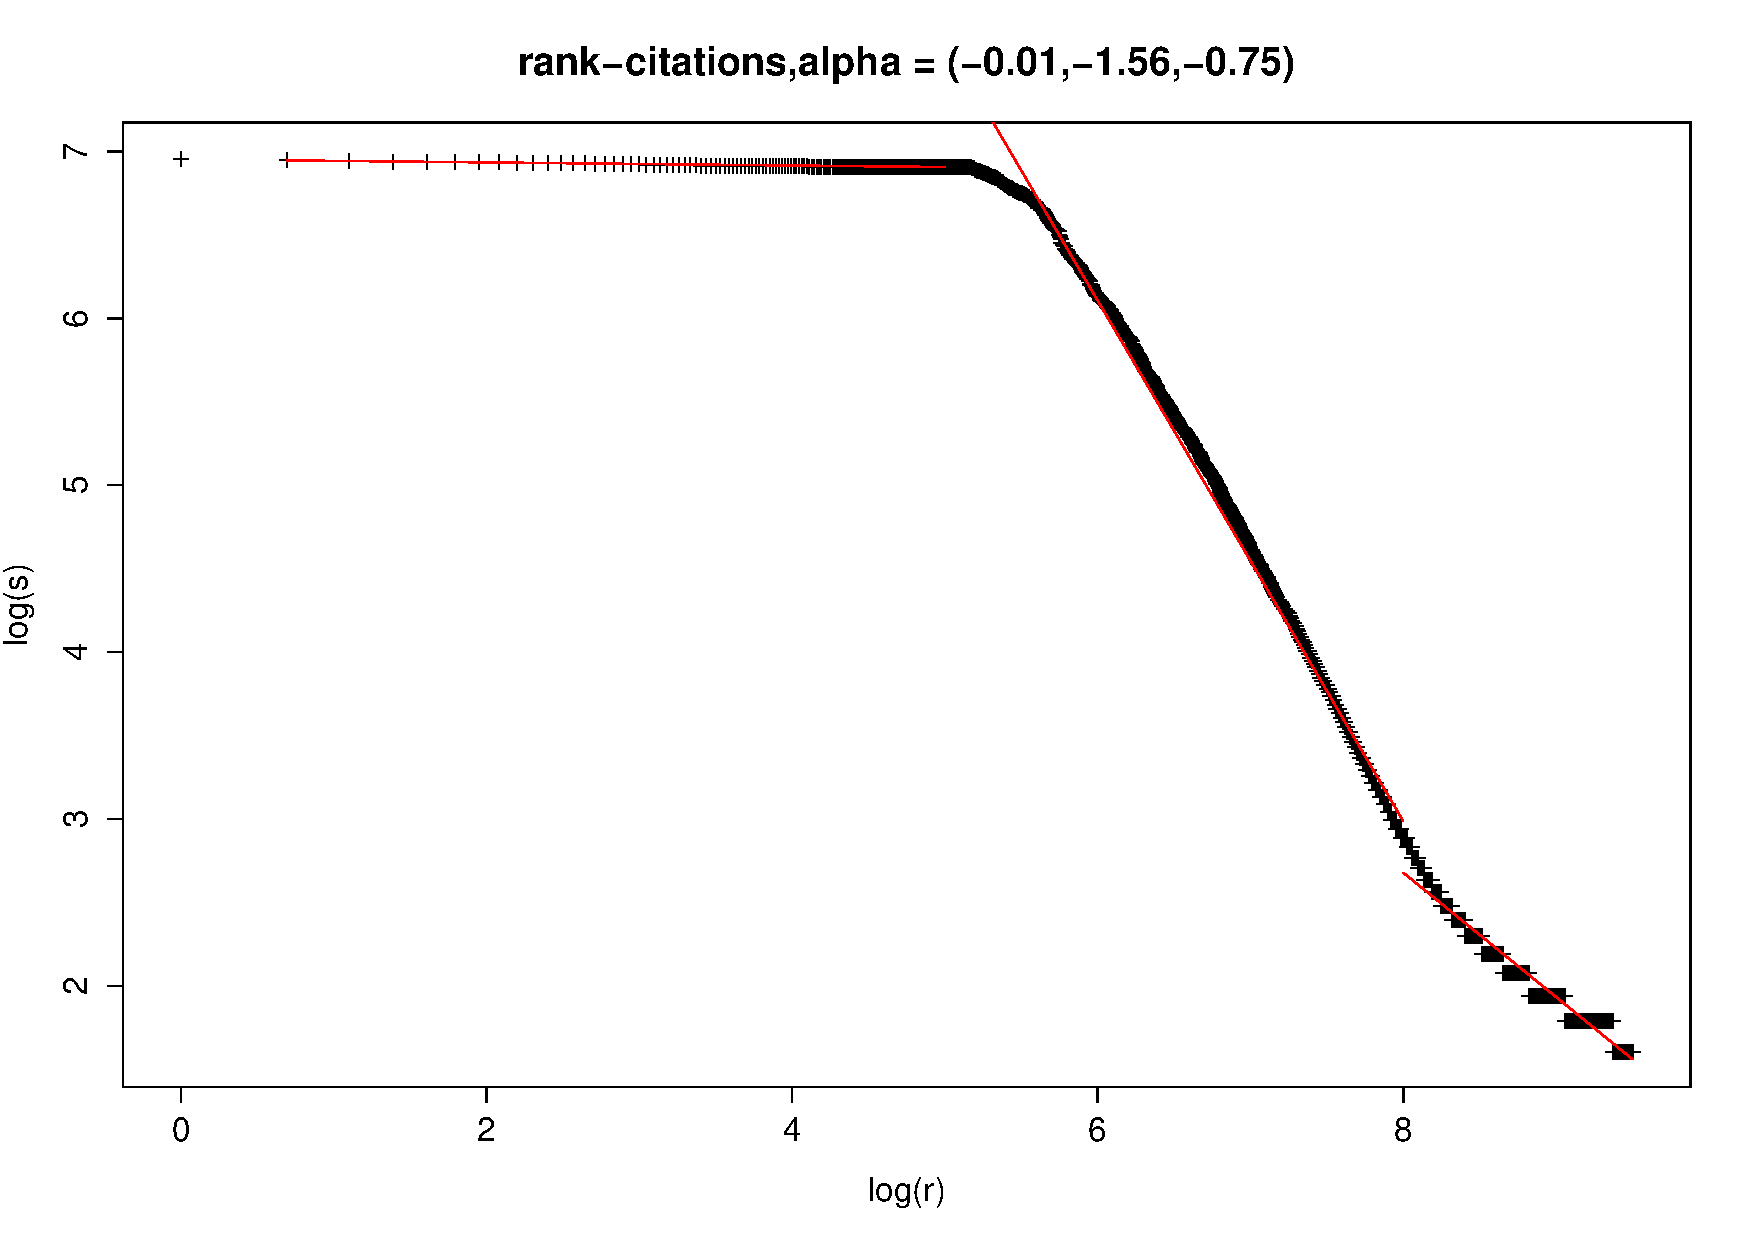
\includegraphics[width=0.5\textwidth]{figures/rank-size-all}

\textit{Gauche : Cyberg{\'e}o ; Droite : Ensemble du r{\'e}seau}

}


\jframe{Clustering}{
Composante g{\'e}ante : plus de 99\% des noeuds.
\medskip

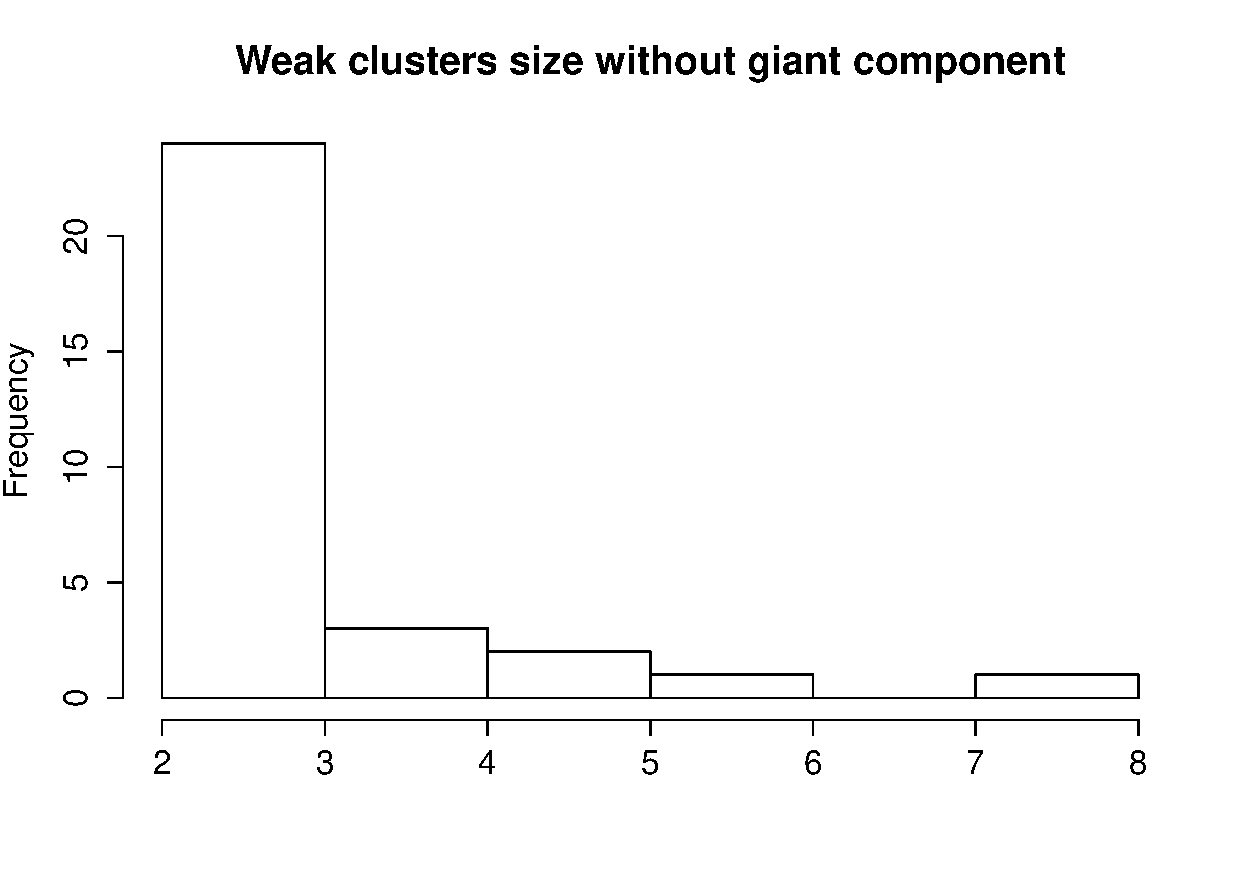
\includegraphics[width=0.5\textwidth]{figures/clusterSize}
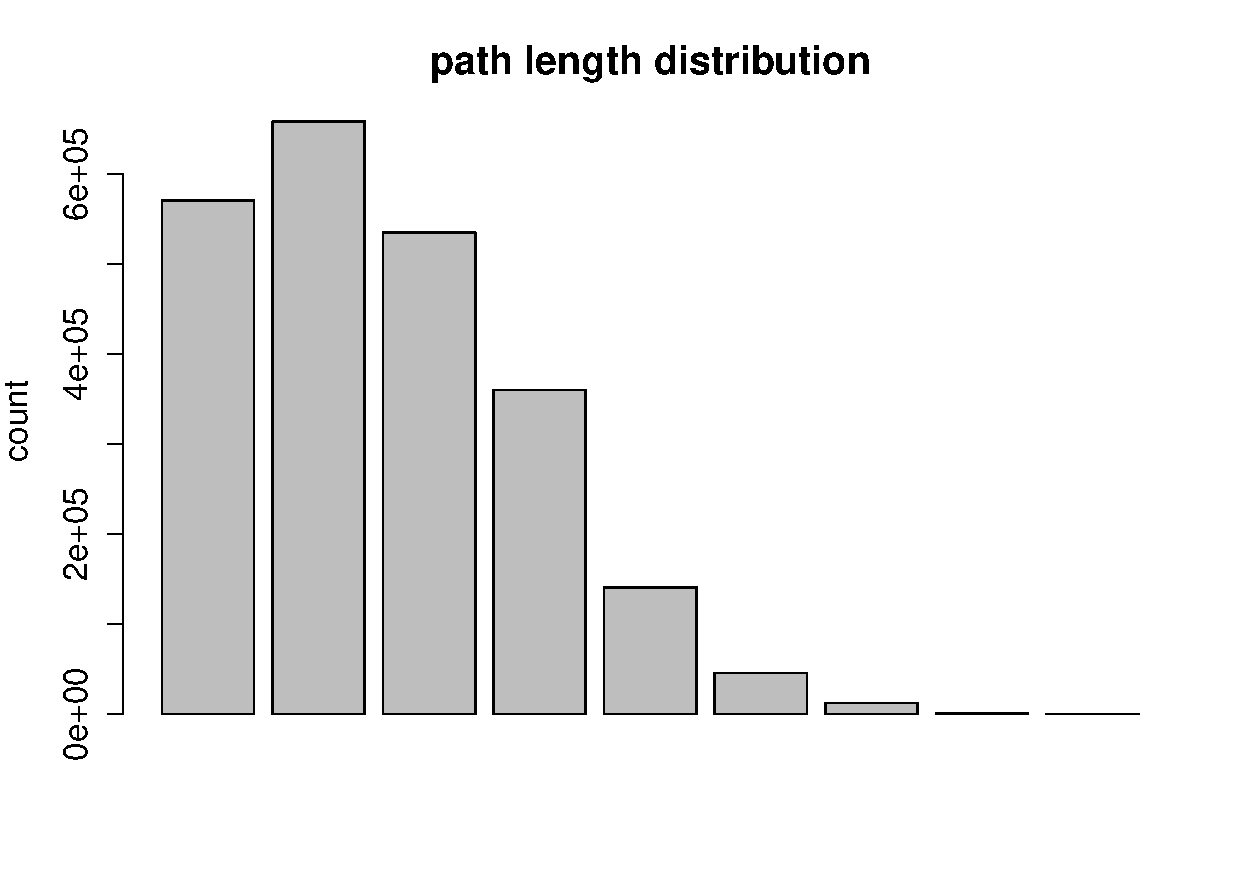
\includegraphics[width=0.5\textwidth]{figures/pathlength}
}



\jframe{Centralit{\'e}}{

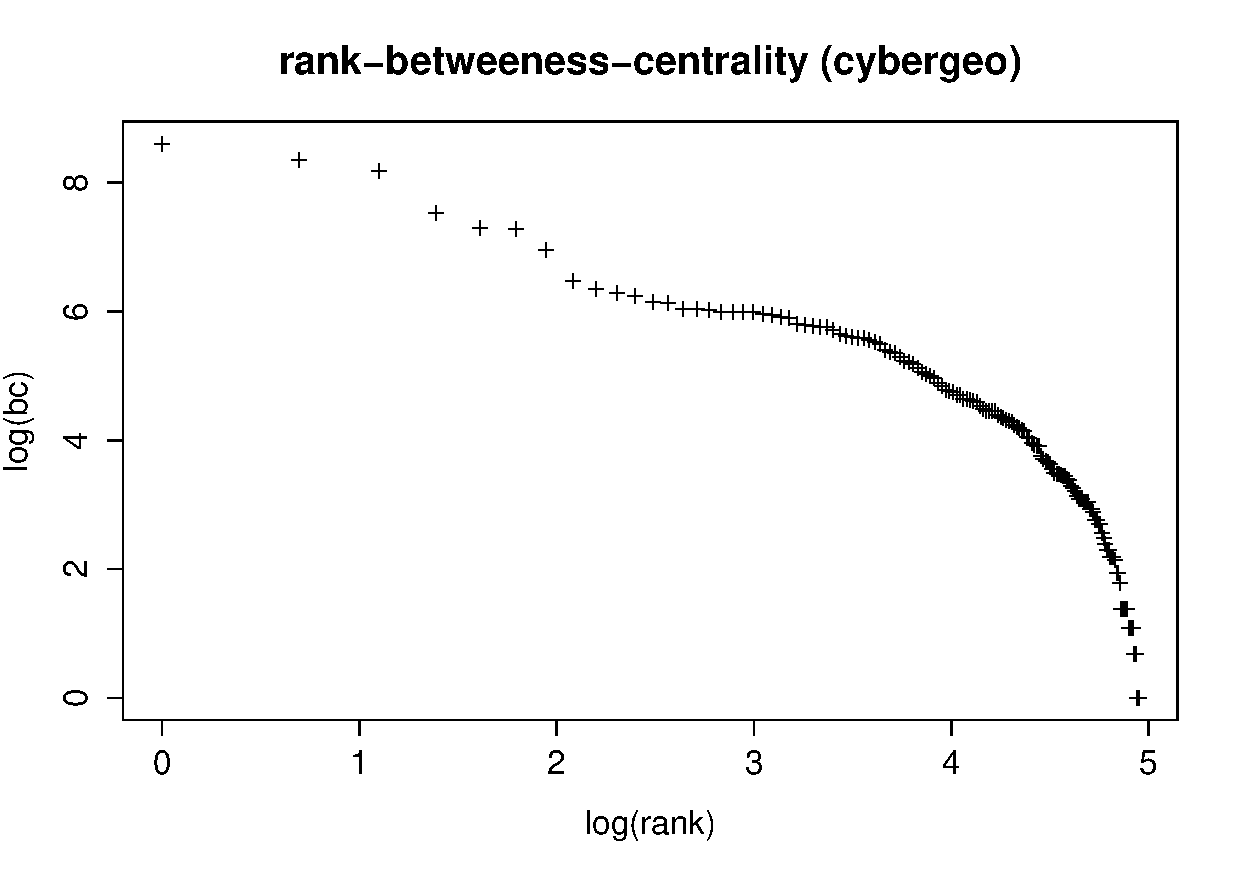
\includegraphics[width=0.5\textwidth]{figures/betweeness-cyb}
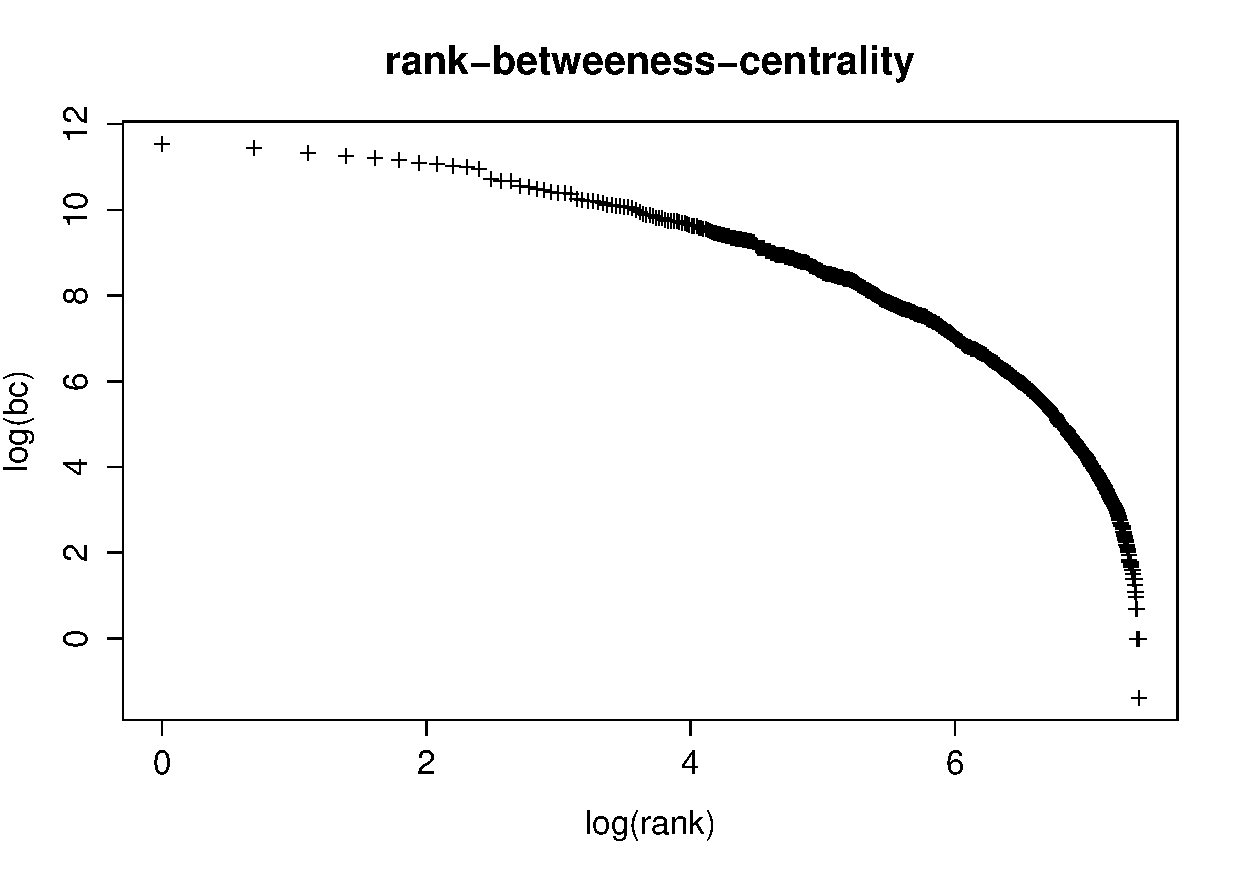
\includegraphics[width=0.5\textwidth]{figures/betweeness}

\textit{Centralit{\'e}s faibles (rq : impossibilit{\'e} des clusters forts pour des citations car causalit{\'e} temporelle). Gauche : Cyberg{\'e}o ; Droite : Ensemble du r{\'e}seau}

}

\jframe{Cliques}{

\textit{viz cliques}

}



%
%\section{Suite de l'étude}
%
%
%\jframe{Suite}{
%\begin{itemize}
%\item Analyse th{\'e}matique cibl{\'e}e des communaut{\'e}s/cliques
%\item Analyses diachroniques
%\item Collection des textes des \textit{abstract} pour l'ensemble du corpus
%\item Construction du r{\'e}seau s{\'e}mantique ; d{\'e}tection de disciplines par communaut{\'e}s.
%\item Croisement des deux couches pour extraire positionnement et importance disciplinaire de cyberg{\'e}o
%\end{itemize}
%
%}
%


\subsection{R{\'e}seau s{\'e}mantique}


\jframe{R{\'e}seau s{\'e}mantique}{


\textbf{R{\'e}seau s{\'e}mantique.} Collection des r{\'e}sum{\'e}s/ann{\'e}es/auteurs/mots-cl{\'e}s pour les 400000 r{\'e}f{\'e}rences via l'API Mendeley
$\rightarrow$ $\sim 215000$ r{\'e}f{\'e}rences avec donn{\'e}es compl{\`e}tes.

\textbf{Statistiques}

\textit{Langues :} anglais 206607, francais 4109, espagnol 2029, allemand 892, portugais 891, n{\'e}erlandais 124, autres 182

\textit{Repartitions par ann{\'e}es : }
\centering

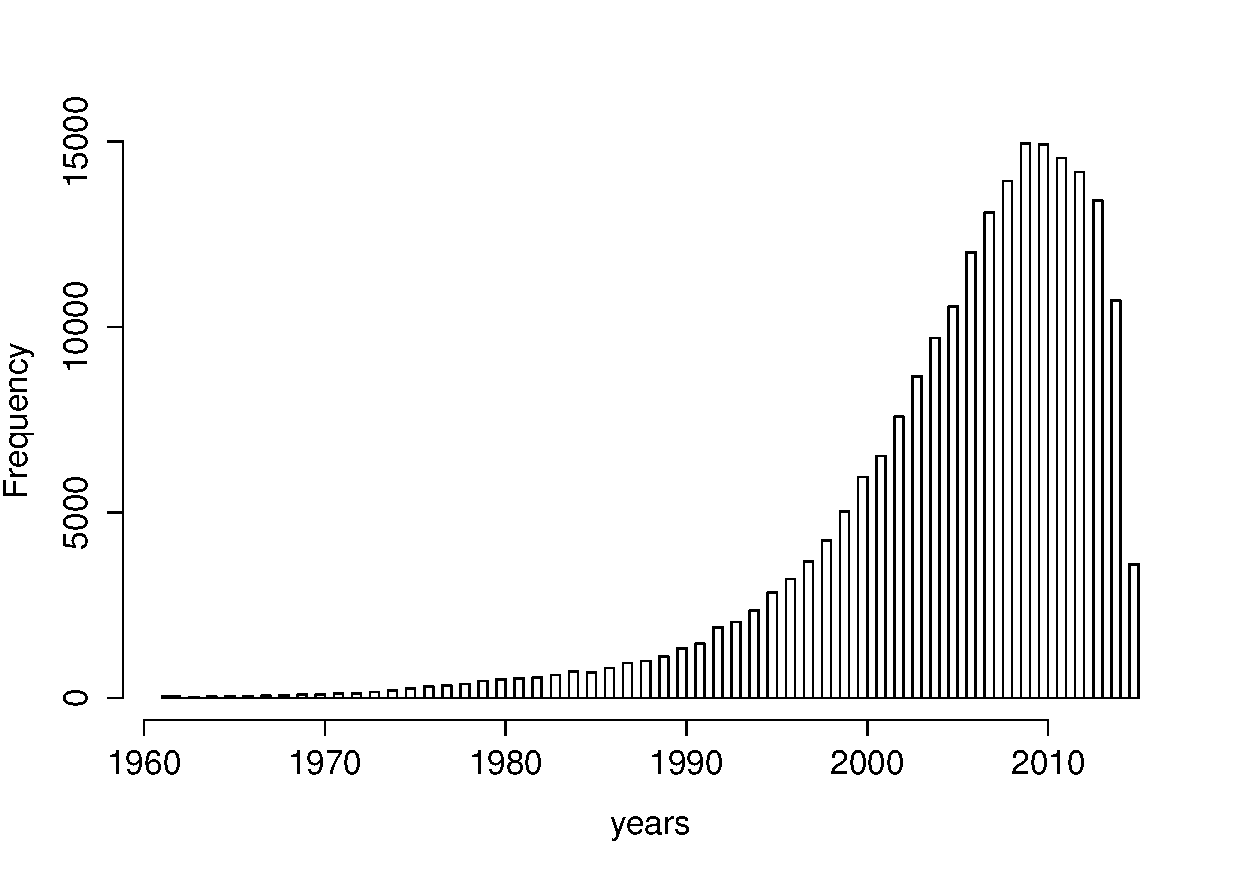
\includegraphics[width=0.3\textwidth,height=0.3\textheight]{figures/years}

}



\jframe{Extraction des mots-cl{\'e}s brute}{

\textit{Text-mining en python avec \texttt{nltk}~\cite{bird2006nltk}}, m{\'e}thode adapt{\'e}e de~\cite{chavalarias2013phylomemetic}

\begin{itemize}
\item Detection de la langue par \textit{stop-words} (mots vides de sens)
\item Parsing et tokenizing (isolation des mots) /pos-tagging (fonction des mots) /stemming (extraction de la racine) effectu{\'e}s diff{\'e}remment selon la langue :
\begin{itemize}
\item Anglais : pos-tagger int{\'e}gr{\'e} {\`a} \texttt{nltk}, combin{\'e} {\`a} un \emph{PorterStemmer}
\item Fran\c{c}ais ou autre : utilisation de \texttt{TreeTagger}~\cite{schmid1994probabilistic}
\end{itemize}
\item Selection des \emph{n-grams} potentiels (avec $1 \leq n \leq 4$) : anglais $\bigcap \{NN \cup VBG \cup JJ \}$ ;  français  $\bigcap \{NOM \cup ADJ\}$
\item Insertion en base pour extraction quasi-instantanée plus tard (10j $\rightarrow$ 5min)
\end{itemize}

}


\jframe{Estimation de la pertinence par bootstrap}{
Estimation exacte de la pertinence via la repartition statistique des co-occurrences (score de $\chi^2$) : \textit{termhood} d{\'e}finie comme
\[
t_i = \sum_{j\neq i}\frac{\left( M_{ij} - \sum_{k}M_{ik} \sum_{k} M_{jk}\right)^2}{\sum_{k}M_{ik} \sum_{k} M_{jk}}
\]


en $\Theta (\sum_i N_i^2)$ ($N_i$ taille des r{\'e}sum{\'e}s) : impossible sur un corpus o{\`u} $\sum_i N_i^2 \simeq N <N_i>^2 \simeq 4\cdot 10^6$

\bigskip


$\rightarrow$ Estimation par \textit{boootstrap} sur des {\'e}chantillons du corpus : moyenne de la \textit{termhood} sur $B$ {\'e}chantillons de taille $C$, avec nombre de mots cl{\'e}s $K_L$


}


\jframe{Bootstrap : convergence de l'estimateur}{
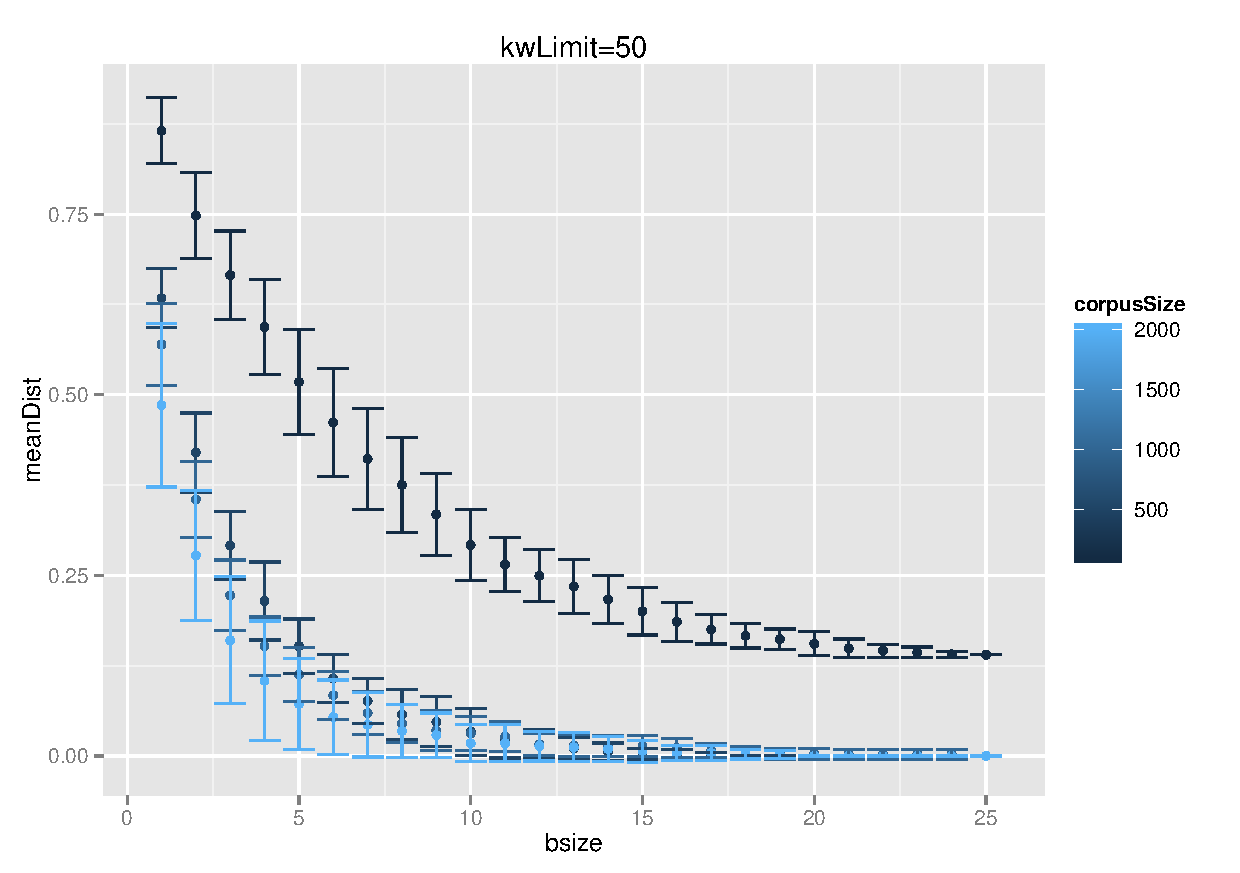
\includegraphics[width=0.55\textwidth,height=0.6\textheight]{figures/kw50}
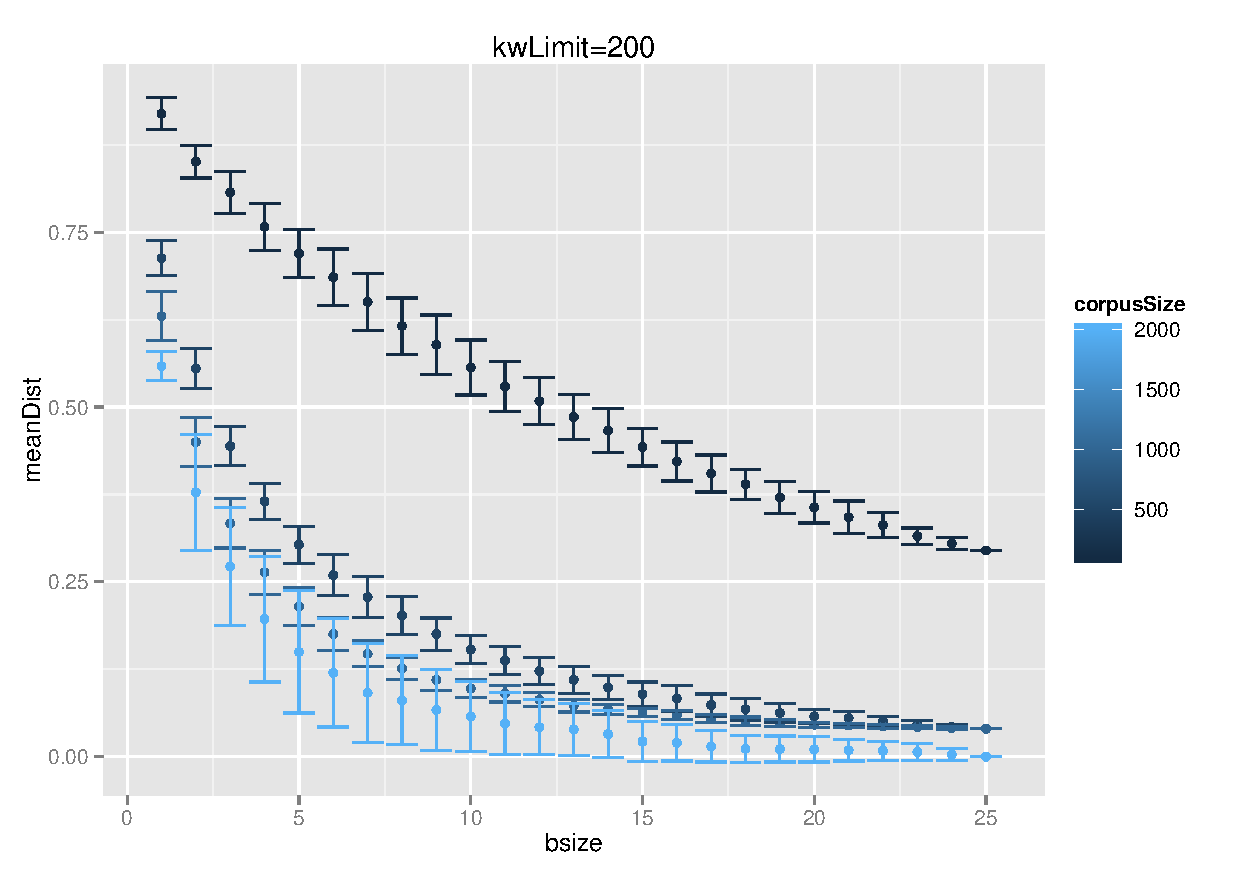
\includegraphics[width=0.55\textwidth,height=0.6\textheight]{figures/kw200}
}


\jframe{Construction du r{\'e}seau s{\'e}mantique}{
\textbf{Noeuds :} Mots-cl{\'e}s avec la plus grande pertinence cumul{\'e}e

\medskip

\textbf{Liens :} Co-occurrences pond{\'e}r{\'e}es

\medskip

Filtrage des liens en dessous d'un seuil ; ajustement manuel de mots parasites

\medskip

Detection de communaut{\'e}s par maximisation de modularit{\'e}~\cite{blondel2008fast} apr{\`e}s suppression des \textit{hubs} (\texttt{model}, \texttt{space}, \texttt{structure}, \texttt{process})

}



\jframe{R{\'e}seau s{\'e}mantique : corpus complet}{
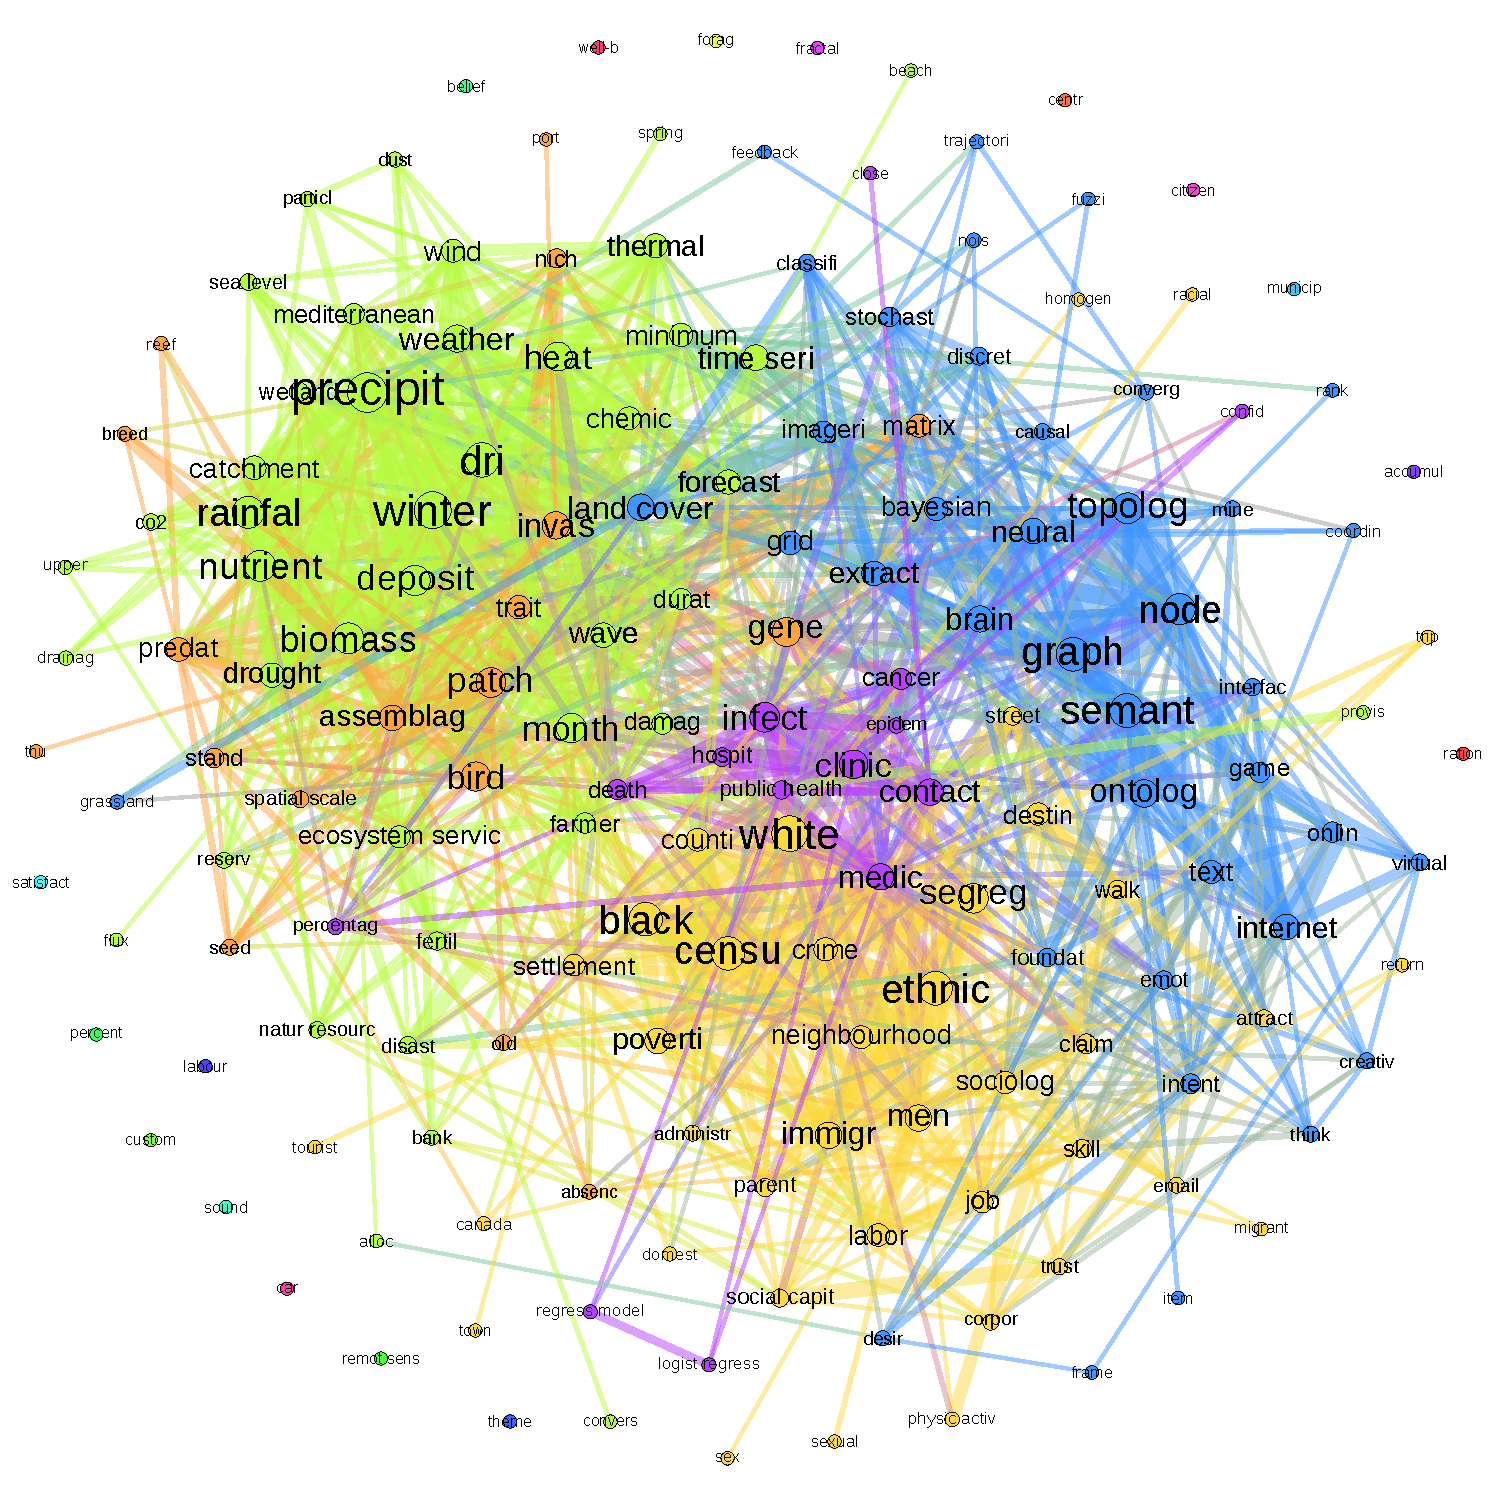
\includegraphics[height=\textheight]{figures/semanticAll}
}


\jframe{R{\'e}seau s{\'e}mantique : corpus cybergeo}{
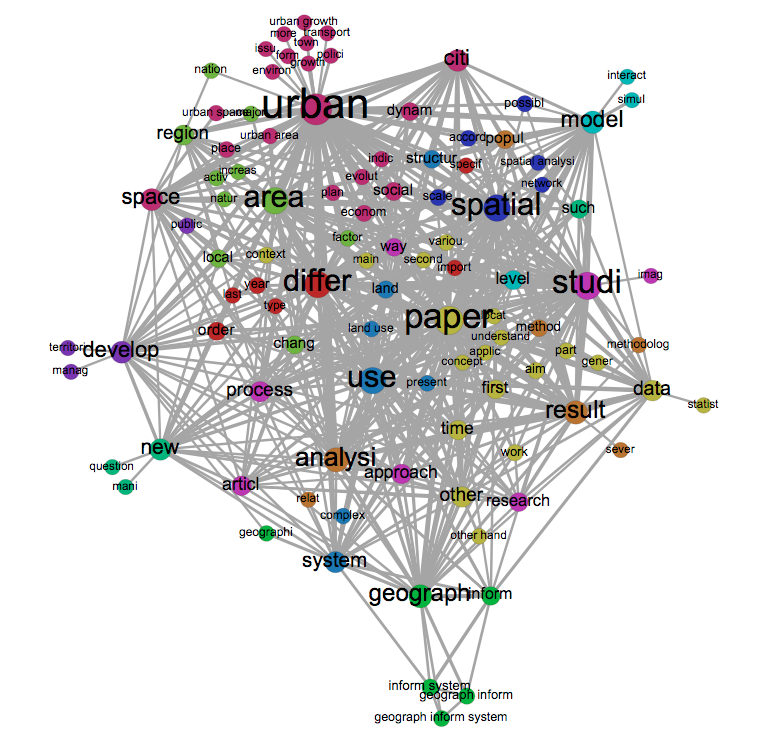
\includegraphics[height=\textheight]{figures/semanticCybergeo}
}




\jframe{Application : degr{\'e} d'interdisciplinarit{\'e}}{
Un article peut être associ{\'e} aux communaut{\'e}s s{\'e}mantiques par ses mots cl{\'e}s : probas $p_i$ pour chaque communaut{\'e}.

Mesure d'interdisciplinarit{\'e} :
\[
o = 1 - \sum p_i^2
\]

}



\jframe{Perspectives}{
\textit{TBW}
}



%
%\jframe{Suite}{
%\begin{itemize}
%\item Bootstrap parallelis{\'e} sur l'ensemble du corpus
%\item Construction du r{\'e}seau : co-occurrences dans les r{\'e}f{\'e}rences\\\textbf{Q : } utilisation des mots-cl{\'e}s des m{\'e}tadonn{\'e}es ? si oui filtrage sur fr{\'e}quence ? test avec/sans
%\item D{\'e}tection de disciplines par communaut{\'e}s dans le r{\'e}seau s{\'e}mantique
%\item Croisement des deux couches pour extraire positionnement et importance disciplinaire de Cyberg{\'e}o
%\end{itemize}
%
%}
%
%\jframe{R{\'e}sultats attendus}{
%\begin{itemize}
%\item Couche des citations : analyse plus fines, cliques et communaut{\'e}s
%\item Interdisciplinarit{\'e} au premier ordre : positionnement de cybergeo dans les cluster s{\'e}mantiques (un article pouvant {\^e}tre vu comme un vecteur de propbabilit{\'e}s d'appartenance aux disciplines)
%\item Interdisciplinarit{\'e} au second ordre : liens de citation autour de cybergeo vers les diff{\'e}rentes disciplines
%\item Comparaison des structures de communaut{\'e} : coefficient de clustering inter-couches ; donne tendance g{\'e}n{\'e}rale
%\end{itemize}
%
%}
%
%



%%%%%%%%%%%%%%%%%%%%%%%%%%%%%%%%
\begin{frame}[allowframebreaks]
\frametitle{References}
\bibliographystyle{apalike}
\bibliography{/Users/Juste/Documents/ComplexSystems/CityNetwork/Biblio/Bibtex/CityNetwork,/Users/Juste/Documents/ComplexSystems/CityNetwork/Docs/Papers/Cybergeo/Biblio/cybergeo}
\end{frame}
%%%%%%%%%%%%%%%%%%%%%%%%%%%%%%%%







\end{document}
